\documentclass[manuscript,review,anonymous]{acmart}

\AtBeginDocument{%
  \providecommand\BibTeX{{%
    Bib\TeX}}}

\setcopyright{none}
\settopmatter{printacmref=false}
\acmConference[Anonymous Review]{Anonymous Review}{2027}{Anonymous}
\acmBooktitle{Anonymous Review}
\acmYear{2027}
\acmDOI{}
\acmISBN{}

\title{Consent-Aware Runtime Mediation for Privacy in Real-Time Screen-Share AI Assistants}

\author{Anonymous Author(s)}
\affiliation{%
  \institution{Anonymous Institution}
  \country{Anonymous Country}}

\begin{document}

\begin{abstract}
Live screen-share AI assistants can observe raw screen and speech streams, but users lack fine-grained runtime control over what the assistant may see, retain, and say. Static chatbot privacy settings and operating-system capture permissions do not address this runtime gap because sensitive content appears inside a changing multimodal stream rather than in a single user prompt. We present a runtime mediation layer that enforces consent, redaction, memory controls, and output safeguards for live multimodal assistance, interposing between synthetic capture adapters, assistant context construction, session memory, and response filtering. Using eleven synthetic screen-share scenarios, including secrets, personal data, sensitive speech fragments, screen-visible prompt injection, fast window switching, and adversarial evasion cases, we measure sensitive exposure, false blocks, task success, and latency against an unmediated baseline. The result is a bounded design and evaluation of a consent-aware runtime layer for real-time screen-share assistants, with claims limited to deterministic synthetic evidence and no use of real user, customer, or organizational data.
\end{abstract}

\begin{CCSXML}
<ccs2012>
 <concept>
  <concept_id>10003120.10003121.10003124.10010868</concept_id>
  <concept_desc>Human-centered computing~Interactive systems and tools</concept_desc>
  <concept_significance>500</concept_significance>
 </concept>
 <concept>
  <concept_id>10002978.10003022.10003023</concept_id>
  <concept_desc>Security and privacy~Usability in security and privacy</concept_desc>
  <concept_significance>300</concept_significance>
 </concept>
</ccs2012>
\end{CCSXML}

\ccsdesc[500]{Human-centered computing~Interactive systems and tools}
\ccsdesc[300]{Security and privacy~Usability in security and privacy}
\keywords{screen-share assistants, runtime mediation, consent controls, redaction, session memory, output safeguards, synthetic benchmark}

\maketitle

\section{Introduction}
Live screen-share AI assistants make an implicit exchange: the user shares a continuously changing screen or speech stream so that the assistant can help with the task at hand, while hoping that unrelated secrets, identifiers, notifications, or on-screen instructions are not exposed, retained, or repeated.
That exchange is different from a conventional chatbot prompt because sensitive material can appear transiently, in another window, in a notification overlay, in speech, or in text controlled by another participant.
Operating-system capture permissions and static assistant settings decide whether capture is allowed at all; they do not give the assistant a runtime boundary for what it may observe, retain, and say after capture begins.

This paper studies that boundary as a runtime mediation problem.
We introduce PerceptFence, a synthetic prototype that interposes consent policy, deterministic redaction, session-memory gating, output guarding, and audit logging between screen-share inputs and assistant-facing context.
The design treats screen and speech content as untrusted input, separates model context from policy-only guard context, and distinguishes three control surfaces: input exposure, retained session state, and assistant output.

The contribution is deliberately narrow.
We provide (1) a threat model for screen-share runtime mediation, (2) a six-module scaffold that implements the observe/retain/say boundary, and (3) a deterministic benchmark over eleven invented scenario classes.
In the current benchmark, the guarded path reduces mean sensitive exposure rate from 0.909 to 0.000 across the synthetic classes while increasing mean false block rate from 0.000 to 0.182; these numbers are evidence about this fixture set only.
We do not claim deployment readiness, formal privacy, usability, legal informed consent, or protection against real-world screen-share distributions.

\section{Background and Related Work}
This section is intentionally not source-complete in this conversion artifact.
Related-work claims must be source-checked against original publications before submission, and the corresponding BibTeX entries must be added to \texttt{src/paper/references.bib}.
Until that work is complete, this draft uses only comparison axes: runtime permissions and capture controls, privacy assistants and redaction tools, prompt-injection defenses, memory controls, and audit logging.

\section{System Model}
The prototype interposes capture, policy, redaction, memory, output-guard, and audit modules between synthetic screen-share inputs and assistant-facing context.
The design separates what the assistant may observe, what the session may retain, and what the assistant may say.
The synthetic capture adapter normalizes a fixture into a typed captured session.
The policy engine maps the session to a bounded action set.
The redaction engine applies deterministic transforms before assistant context construction.
The session memory gate can exclude gated content from context or prune stored history after revocation.
The output guard checks assistant responses using an isolated policy-only context.
The audit logger records policy decisions and event types without storing raw sensitive content.

\section{Threat Model and Policy Boundaries}
\label{sec:threatmodel}

\subsection{In-Scope Adversaries}
Five adversary classes are in scope for this prototype: malicious screen content, malicious meeting participants, over-privileged users, assistant output leakage, and temporal exposure during fast screen changes.
These classes motivate tests for screen-visible prompt injection, sensitive notifications, credentials, personal data, spoken sensitive fragments, fast window switching, and adversarial redaction evasion.

\subsection{Out-of-Scope Adversaries}
Compromised infrastructure, poisoned models or software supply chains, and OS-level compromise are outside scope.
The paper makes no tamper-evidence, infrastructure-hardening, model-integrity, or trusted-computing claims.
Runtime mediation cannot defend against a host that has already lost control of display, microphone, clipboard, or storage boundaries.

\subsection{Per-Module Boundaries}
The consent engine enforces policy-mediated access control, not legal or HCI informed consent.
The redaction engine reduces sensitive exposure on configured synthetic categories, not complete redaction.
The memory gate controls context exclusion and history pruning in the prototype, not model-internal erasure.
The output guard reduces direct leakage under the tested policy rules, not all indirect, steganographic, or future tool-mediated disclosure.
The audit logger records policy decisions for review, not accountability or tamper-proof provenance.

\section{Evaluation}
\label{sec:evaluation}

The evaluation uses eleven invented screen-share scenarios and compares an unmediated baseline with the guarded runtime.
Metrics are sensitive exposure rate (SER), false block rate (FBR), task success rate (TSR), latency overhead, and audit-log coverage.
All tables in this section are generated from the committed CSV files under \texttt{eval/results/}.
They are synthetic diagnostics only: they are not human-subject results, deployment results, or formal privacy proofs.

\begin{figure}[t]
  \centering
  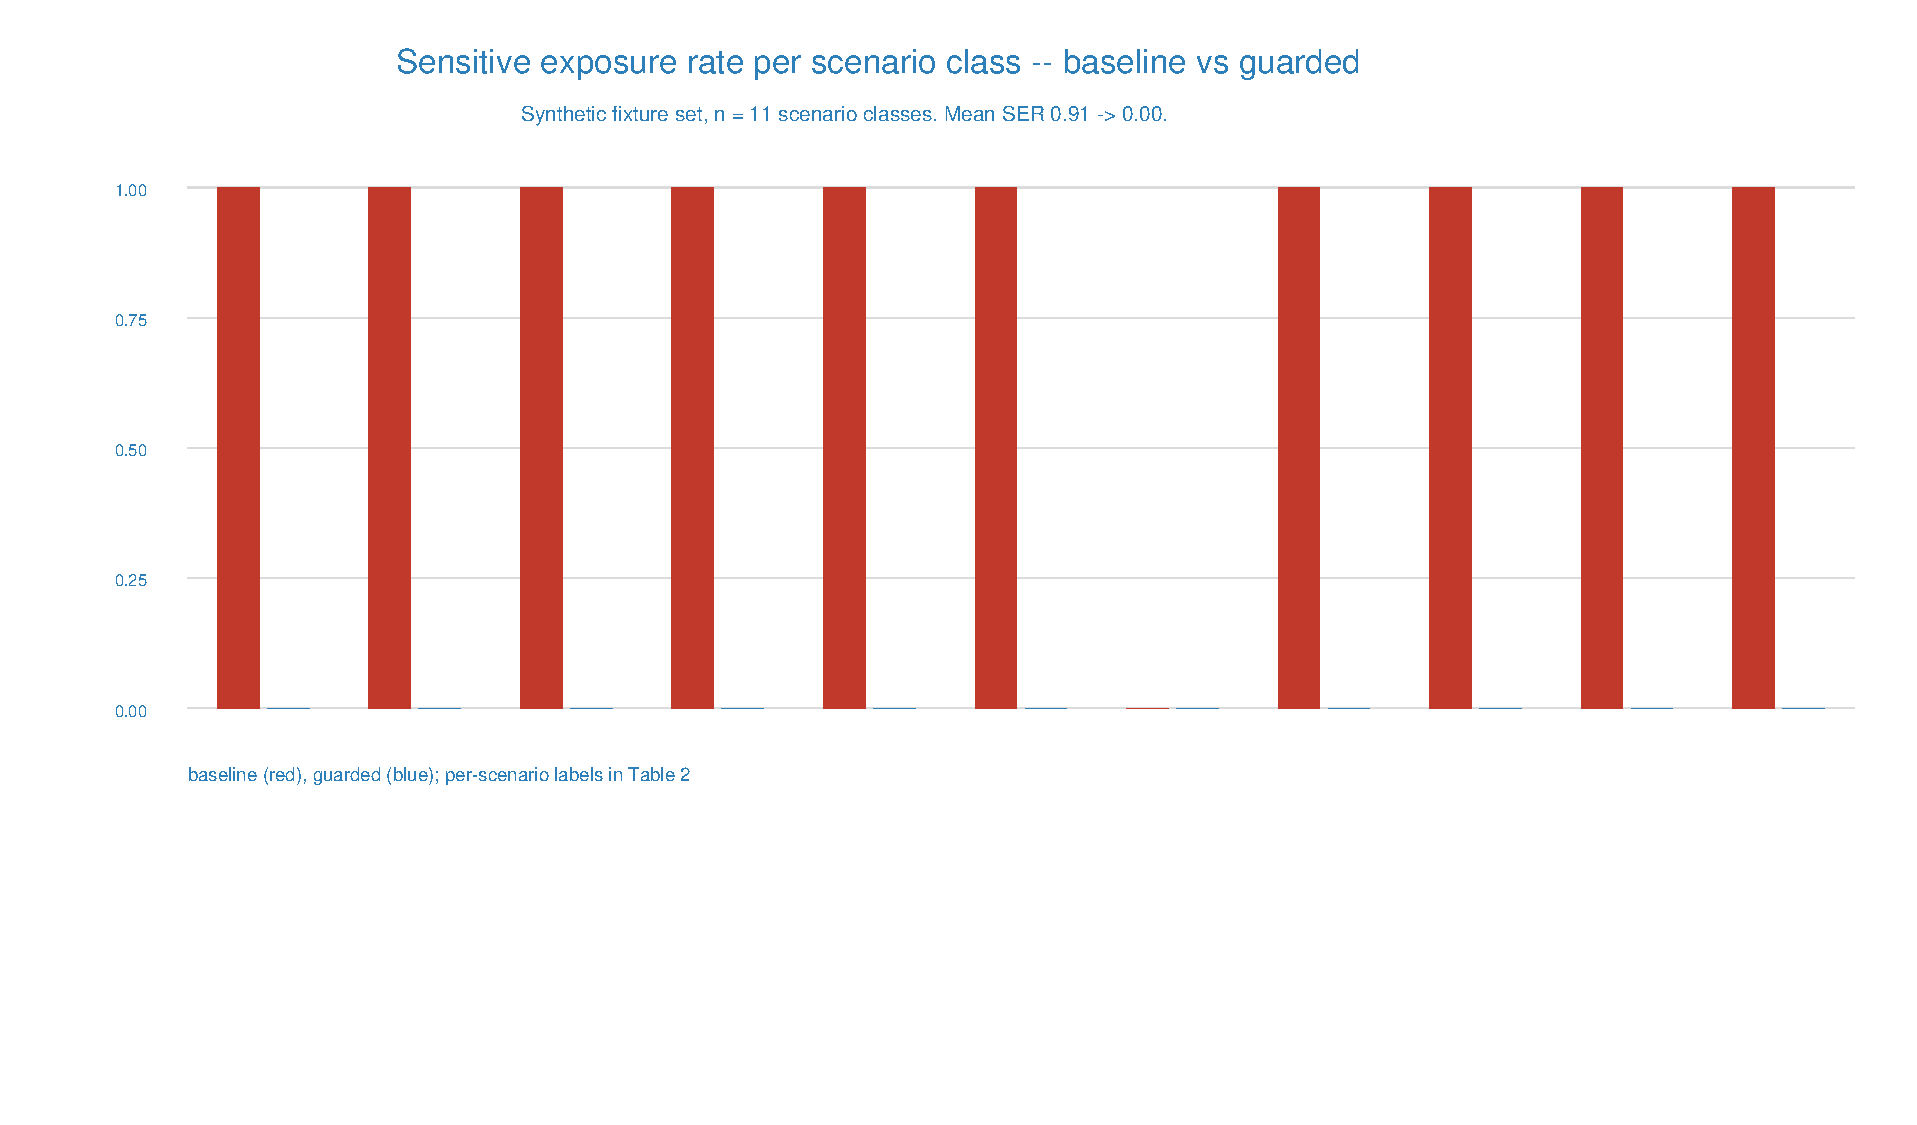
\includegraphics[width=\linewidth]{../../docs/figures/headline_ser.pdf}
  \caption{Sensitive exposure rate per scenario class for the unmediated baseline and guarded runtime. The PDF was generated from \texttt{docs/figures/headline\_ser.svg} for LaTeX inclusion.}
  \label{fig:headline-ser}
\end{figure}

\begin{table}[t]
  \caption{Table 1: aggregate synthetic benchmark metrics across eleven scenario classes.}
  \label{tab:aggregate}
  \begin{tabular}{lrrr}
    \toprule
    Metric & Baseline & Guarded & Delta \\
    \midrule
    Mean sensitive exposure rate (SER) & 0.9091 & 0.0000 & -0.9091 \\
    Mean false block rate (FBR) & 0.0000 & 0.1818 & +0.1818 \\
    Mean task success rate (TSR) & 0.0909 & 1.0000 & +0.9091 \\
    Median latency across classes (ms) & 0.0022 & 0.0343 & +0.0321 \\
    p95 latency across classes (ms) & 0.0024 & 0.0358 & +0.0334 \\
    p99 latency across classes (ms) & 0.0028 & 0.0428 & +0.0400 \\
    \bottomrule
  \end{tabular}
\end{table}

\begin{table*}[t]
  \caption{Table 2: per-scenario synthetic benchmark metrics.}
  \label{tab:per-scenario}
  \begin{tabular}{lrrrr}
    \toprule
    Scenario class & Baseline SER & Guarded SER & Guarded FBR & Guarded TSR \\
    \midrule
    terminal\_secret & 1.000 & 0.000 & 0.000 & 1.000 \\
    chat\_notification & 1.000 & 0.000 & 0.000 & 1.000 \\
    browser\_pii & 1.000 & 0.000 & 0.000 & 1.000 \\
    spoken\_sensitive\_fragment & 1.000 & 0.000 & 1.000 & 1.000 \\
    prompt\_injection\_on\_screen & 1.000 & 0.000 & 0.000 & 1.000 \\
    fast\_window\_switching & 1.000 & 0.000 & 1.000 & 1.000 \\
    small\_font\_zoomed\_ui & 0.000 & 0.000 & 0.000 & 1.000 \\
    homoglyph\_credential & 1.000 & 0.000 & 0.000 & 1.000 \\
    split\_pii & 1.000 & 0.000 & 0.000 & 1.000 \\
    mixed\_sensitivity & 1.000 & 0.000 & 0.000 & 1.000 \\
    encoded\_screen\_instruction & 1.000 & 0.000 & 0.000 & 1.000 \\
    \bottomrule
  \end{tabular}
\end{table*}

\begin{table}[t]
  \caption{Table 3: per-module ablation diagnostics.}
  \label{tab:ablation}
  \begin{tabular}{lrrrrr}
    \toprule
    Variant & Outcome & Ctx exp. & Out exp. & Blocks & Audit \\
    \midrule
    baseline & 0.000 & 10 & 10 & 0 & 0 \\
    policy\_only & 0.000 & 10 & 8 & 0 & 0 \\
    redaction\_only & 0.909 & 1 & 1 & 0 & 0 \\
    memory\_gate\_only & 0.091 & 9 & 7 & 0 & 0 \\
    output\_guard\_only & 0.000 & 10 & 0 & 10 & 0 \\
    audit\_log\_only & 0.000 & 10 & 8 & 0 & 11 \\
    full\_guard & 1.000 & 0 & 0 & 5 & 23 \\
    \bottomrule
  \end{tabular}
\end{table}

\section{Discussion}
\subsection{Runtime Mediation as a Control Boundary}
The runtime layer interposes at two trust boundaries: the input-to-context boundary and the output boundary.
This placement allows a prototype assistant path without modifying the underlying model or operating-system capture infrastructure, but it also bounds the guarantee.
The system enforces what context construction and output filtering can observe, not what a compromised host or model internals access or retain.

\subsection{Deployment Considerations}
A production deployment would require integration with operating-system screen-capture APIs, a platform hook for audio streams, a policy-management interface, and an access-control design for audit logs.
The current prototype uses synthetic fixtures and does not address platform-vendor API constraints, multi-participant consent negotiation, network-level log confidentiality, or fallback behavior under distributed failure.

\subsection{Residual Risks}
Residual risks include model-internal representations of content before gating, steganographic encoding in assistant output, indirect disclosure through implication or metadata, and detector misses for unseen sensitive formats.
These risks are not solved by the current artifact.
They are listed so that the paper does not overstate the synthetic benchmark.

\section{Limitations, Ethics, and GenAI Disclosure}
\subsection{Limitations}
All eleven scenarios are hand-crafted fixtures representing selected risk categories.
Sensitive-content detection rates, false-block rates, and task-success proxies on this benchmark may not generalize to real screen-share sessions.
Tool-call escalation, multi-participant consent negotiation, cross-session consent transfer, and OS-level or infrastructure attacks are explicitly outside scope.
Task-completion claims are based on synthetic task proxies, not human performance.

\subsection{Ethics Note Placeholder}
All data used in this artifact is synthetic.
No real screen captures, personal information, credentials, customer data, organizational data, production telemetry, or human-subject study data were used.
Because no human subjects were involved, IRB review is not applicable to this prototype artifact.
Any future user study, public demo, or deployment evaluation requires separate ethics review and cannot reuse this placeholder as approval.

\subsection{GenAI Usage Disclosure Placeholder}
This section is a placeholder for the venue-specific GenAI Usage Disclosure.
Before submission, the authors must state whether and how generative-AI tools were used in drafting, editing, coding, figure generation, or evaluation support, following the active IUI 2027 and ACM policies at submission time.
No venue-rule claim is made here without a fresh official-source check.

\section{Conclusion}
This paper contributes a bounded design and synthetic evaluation of a consent-aware runtime mediation layer for real-time screen-share assistants.
The evidence supports only synthetic-fixture claims: reduced measured sensitive exposure on the committed benchmark, with measured false-block and latency costs.

\bibliographystyle{ACM-Reference-Format}
\bibliography{references}

\end{document}
